% Template for ICIP-2015 paper; to be used with:
%          spconf.sty  - ICASSP/ICIP LaTeX style file, and
%          IEEEbib.bst - IEEE bibliography style file. cambio para probar adsfasfasfasfsf
% --------------------------------------------------------------------------
\documentclass[spanish,twocolumn]{article}
\usepackage{spconf,amsmath,graphicx}
\usepackage{mathptmx}
\usepackage{mathtools}
\usepackage{amsmath}
\usepackage{mathrsfs}
\usepackage{amssymb}
\usepackage{amsfonts}
\usepackage[utf8]{inputenc}
\usepackage{babel}
\usepackage{color}
\usepackage[]{algorithm}
\usepackage{algpseudocode}
\usepackage{multicol}
\usepackage{caption,setspace}
\usepackage{subfig}
\usepackage{graphicx}

%\algrenewcommand\algorithmicif{\textbf{si}}
%\algrenewcommand\algorithmicend{\textbf{fin}}
%\algrenewcommand\algorithmicfor{\textbf{para}}
%\algrenewcommand\algorithmicdo{\textbf{hacer}}
%\algrenewcommand\algorithmicwhile{\textbf{mientras}}
%\algrenewcommand{\algorithmicrequire}{\textbf{Entrada:}}
%\algrenewcommand{\algorithmicensure}{\textbf{Salida:}}
%\selectlanguage{spanish}
% Example definitions.
% --------------------
\def\x{{\mathbf x}}
\def\L{{\cal L}}

\setlength{\textfloatsep}{10pt plus 1.0pt minus 3.0pt}

% Title.
% ------
\title{PARAMETER TUNING OF CLAHE BASED ON MULTI-OBJECTIVE OPTIMIZATION TO ACHIEVE DIFFERENT CONTRAST LEVELS IN MEDICAL IMAGES}
%\title{OPTIMIZACIÓN MULTIOBJETIVO PARA LA MEJORA DEL CONTRASTE BASADA EN CLAHE.}
%
% Single address.
% ---------------
\name{Luis G. Moré, Marcos A. Brizuela, Horacio Legal Ayala, Diego P. Pinto-Roa, José Luis Vázquez Noguera}
\address{Facultad Politécnica - Universidad Nacional de Asunción}
%
% For example:
% ------------
%\address{School\\
%	Department\\
%	Address}
%
% Two addresses (uncomment and modify for two-address case).
% ----------------------------------------------------------
%\twoauthors
%  {A. Author-one, B. Author-two\sthanks{Thanks to XYZ agency for funding.}}
%	{School A-B\\
%	Department A-B\\
%	Address A-B}
%  {C. Author-three, D. Author-four\sthanks{The fourth author performed the work
%	while at ...}}
%	{School C-D\\
%	Department C-D\\
%	Address C-D}
%
\begin{document}
%\ninept
%
\maketitle
%
\begin{abstract}
In certain medical images, it is possible to achieve contrast enhancement at different levels, in order to highlight different structures present therein. This could be useful to medical specialists to perform more specific diagnoses, in chest radiographs and mammograms, where it is possible to highlight different details when contrast is enhanced. Parameter tuning for Contrast Limited Adaptive Histogram Equalization(CLAHE) using a multi-objective meta-heuristic (SMPSO) is proposed, where the objective functions are the maximization of the amount of information available (via Entropy) and minimization of distortion in the resulting images (Structural Similarity Index, SSIM) simultaneously. The results show a set of solutions or Pareto Set, which represents images with different contrast levels and different levels of commitment between Entropy and Structural Similarity Index, which shows that these objectives are contradictory. These enhanced images provide useful information for decision making of specialists.

\end{abstract}
%
\begin{keywords}
SMPSO, CLAHE, Entropy, SSIM, Contrast Enhancement, Multiobjective Optimization.
\end{keywords}
%
\section{INTRODUCTION}
\label{sec:intro}

Improve contrast of medical images is a very important task in order to emphasize and maintain the features present within them. Radiographs show particular contrast features, such as in chest radiography and mammograms, because there might be notorious contrast differences because of the attenuation characteristics of X-Rays \cite{chang1998image}. 

Important efforts are devoted to achieve Contrast Enhancement and automatically assess the quality of the results \cite{LTG,6963384,1658094,7056527}. Local improvement approaches prove to be extremely useful when enhancing details in medical images, and there are various proposals focused on improving radiography contrast \cite{1625082,4712472,5360176}. In our proposal a meta-heuristic for optimization will be used, in order to tune input parameters of the contrast enhancement algorithm described in section \ref{sec:clahe}; in this context, we will get groups of images with different contrast levels, which will be evaluated assessing the provided information gain and distortion introduced by the equalization process (section \ref{sec:metricas}). Obtained images show different relationships between contrast and distortion, in order to highlight different features of the test images, which is useful for analysis performed by the specialist. The literature shows several proposals for improvement based on meta-heuristics, as shown in \cite{Hashemi20101816}, where a Genetic Algorithm is used; in \cite{morebrizuela2014} a similar approach to ours is used, although it focuses on a single objective and only one result is obtained for each original image; or in \cite{Shanmugavadivu2014243} a multi-objective meta-heuristic based on weighted sums is also used; the main difference is that our proposal is implemented more effectively in medical imaging because CLAHE shows satisfactory results in this type of images \cite{reza2004,5360176}, and we obtain a set of non-dominated solutions, which leads to a pure multiobjective optimization approach.

The rest of the paper is organized as follows: In section \ref{sec:clahe} the adopted contrast enhancement algorithm is described briefly; in section \ref{sec:metricas} it is shown the metrics for evaluating results; section \ref{sec:formulacion} formally poses the problem being solved; section \ref{sec:propuesta} shows how the optimization approach is applied to the contrast enhancement algorithm; then in the section \ref{sec:resultadosdiscusion}, the results are discussed, and finally in section \ref{sec:conclusion} the corresponding conclusions are detailed.


\section{Contrast Limited Adaptive Histogram Equalization - CLAHE}
\label{sec:clahe}

This contrast enhancement approach presented in \cite{Zuiderveld:1994:CLA:180895.180940} is an extension of the original Adaptive Histogram Equalization (AHE) algorithm \cite{pizer1987adaptive}; both methods implement equalization based on Contextual Regions whose dimensions are defined by $(\mathcal{R}_x, \mathcal{R}_y)$ to perform equalization in several areas of the image. Inconsistencies between borders are corrected using bilinear interpolation. AHE presents problems of noise amplification, so in CLAHE a limitation is implemented in the contrast through limiting the number of pixels that can achieve certain grayscales within the local histogram; here the {\it Clip Limit} coefficient $\mathcal{C}$ is defined as a factor that is closely related to the contents of the histogram.


\section{EVALUATION METRICS}
\label{sec:metricas}

In order to evaluate the performance of CLAHE, metrics are needed to measure the quality of the resulting images; two coefficients were adopted that are important for comparisons between different results:  {\it Entropy} as a contrast enhancement measure, and {\it Structural Similarity Index} as a measure of image distortion.  

\subsection{Entropy}
\label{ssec:entropia}

The {\it Information Entropy} is a measure of randomness of the image \cite{tsai2008information}. Entropy of the image is defined as:

\begin{equation}\label{eq:entropia}
\mathscr{H}=-\sum_{i=0}^{L-1}\mathcal{P}_i log_2(\mathcal{P}_i) [bits] \quad \mathscr{H} \in \{0,...,log_2(L)\} 
\end{equation}

Where $\mathcal{P}_i$ is the probability of occurrence of gray levels $i$ in the image and $L$ is the maximum grayscale that can be used to represent the image. This metric is interesting because it is strongly associated with the average brightness of the image \cite{108593}; this ratio helps us see how the contrast increases as a result of the transformation of the image.

\subsection{Structural Similarity Index}
\label{ssec:ssim}

The {\it Structural Similarity Index (SSIM)} \cite{wang2004image} is a coefficient that measures the degree of distortion in a resulting image $T$ as a result of applying ontrast enhancement to an original image $I$. $SSIM$ is calculated by blocks, so given two image windows $I_x$ and $T_y$ for the original and resulting images, respectively, the $SSIM$ is defined as shown below:

\begin{equation}\label{eq:ssim}
\resizebox{.9\hsize}{!}
{
$SSIM(I,T)=\frac{(2\mu_{I_x}\mu_{T_y}+C_1)(2\sigma_{I_xT_y}+C_2)}{(\mu_{I_x}^2+\mu_{T_y}^2+C_1)(\sigma_{I_x}^2+\sigma_{T_y}^2+C_2)} \quad SSIM \in [0,1]$
}
\end{equation}

Where $\mu_{I_x}$ is the intensity average of $I_x$; $\mu_{T_y}$ is the intensity average of $T_y$; $\sigma_{I_x}^2$ and $\sigma_{T_y}^2$ are the intensity variances for $I_x$ and $T_y$, respectively; $\sigma_{I_x T_y}$ is the covariance between $I_x$ and $T_y$; $C_1=(K_1L^2)$, $L$ is the dynamic range of intensities of the pixels (256 for a grayscale image of 8 bits) and $K_1 \ll 1$ is a small constant; $C_2=(K_2 L)^2$, and $K_2 \ll 1$; both $C_1$ y $C_2$ are constants that are used to stabilize the division in case the denominator approaches zero.

\begin{algorithm}[H]
    \scriptsize
    \begin{algorithmic}[1]
        \Require Input image $I$, amount of particles $\Omega$, iterations $t_{max}$
        \State Initialize $\omega$, $C_1$, $C_2$, $t=0$, $lower\_limit_1$, $lower\_limit_2$, $lower\_limit_3$, $upper\_limit_1$, $upper\_limit_2$, $upper\_limit_3$, $\mathscr{X}$
        %\For{cada $i$-ésima partícula del enjambre}
        %    \State Inicializar la posición $x_i$ aleatoriamente
        %    \State Inicializar la velocidad $v_i$ a 0
        %    \State ${imagenMejorada}$ = CLAHE(${x_i}$, ${imagenOriginal}$)
        %    \State ${f_i}$ = evaluarAptitud(${imagenOriginal}$, ${imagenMejorada}$)
        %    \State Establecer el mejor individual inicial $p_i$ por el valor inicial $x_i$
        %    \If{$f_i < f_{p_g}$}
        %        \State reemplazar $p_g$ por el valor de $x_i$
        %    \EndIf
        %\EndFor
        \While{$t$ $<$ $t_{max}$}
            \For{every $i$-th particle}
                \State Calculate new velocity $\overrightarrow{v_i}^t$ of the particle  using equations \eqref{eq:psobasico2} and \eqref{eq:restricciondelta}


                \State Calculate new particle position $\overrightarrow{x_i}^t$ using expression \eqref{eq:psobasico}

                \State ${T}$ = CLAHE(${\overrightarrow{x_i}^t}$, ${I}$)
                \State ${f^t_i}$ = $f(I, \overrightarrow{x_i}^t)$%evaluarAptitud(${I}$, ${T}$)
                \If{$f^t_i < f_{\overrightarrow{x}_{p_i}}$}
                    \State replace $\overrightarrow{x}_{p_i}$ by $\overrightarrow{x_i}^t$
                \EndIf
                \If{$ \overrightarrow{x_i} \succ \overrightarrow{x_{g_i}}$  }
                    \State Update $\mathscr{X}$
                \EndIf
                \State $t$ = $t$ + 1
            \EndFor
        \EndWhile
    \Ensure $\mathscr{X}$
    \end{algorithmic}
    \caption{MOPSO-CLAHE}
    \label{alg:pso_clahe}
\end{algorithm}

\section{FORMULATION OF THE PROBLEM POSED}
\label{sec:formulacion}

Given an input image $I$ with $M \times N$ pixels, and a vector $\overrightarrow{x}=(\mathcal{R}_x, \mathcal{R}_y, \mathcal{C})$, where $\mathcal{R}_x$ and $\mathcal{R}_y$ are contextual regions and $\mathscr{C}$ is the {\it Clip Limit}, it is needed to calculate a set of $\mathscr{X}$ solutions, which simultaneously maximize the objectives $f_1$ and $f_2$, as shown below:

\begin{equation}\label{eq:fitness}
    f(I, \overrightarrow{x}) = \{ f_1(I, \overrightarrow{x}), f_2(I, \overrightarrow{x}) \} \qquad f_1,f_2 \in [0,1]
\end{equation}

where:
\begin{itemize}
\item $T$ is the image enhanced by $CLAHE$ using the parameters $\overrightarrow{x}$ applied to $I$; this is $T=CLAHE(\overrightarrow{x},I)$.
\item $f_{1}(I, \overrightarrow{x})=\frac{\mathscr{H}(T)}{log_{2}L}$ is the normalized Entropy of image $T$.
\item $f_{2}(I, \overrightarrow{x})=SSIM(I,T)$ the $SSIM$ between $I$ and $T$.



\end{itemize}

Bounded to:

\begin{itemize}
\item $\mathcal{R}_x \in [2,..,M]$ for the $\mathbb{N}$ numbers.
\item $\mathcal{R}_y \in [2,..,N]$ for the $\mathbb{N}$ numbers.
\item $\mathscr{C} \in (0,1]$ for the $\mathbb{R}$ numbers.
\end{itemize}

\section{PROPOSAL}
\label{sec:propuesta}

The $SMPSO$ \cite{4938830} meta-heuristic is used to calculate the potential solutions $\overrightarrow{x}=(\mathcal{R}_x, \mathcal{R}_y, \mathcal{C})$ at each generation. $SMPSO$ hands a set of solutions $\Omega$ called {\it swarm}, which contains {\it particles} that represent potential solutions. Each particle $\overrightarrow{x_i}$ is updated at each generation $t$ according to the following equation: 

\begin{equation}\label{eq:psobasico}
\overrightarrow{x_i}^t = \overrightarrow{x_i}^{(t-1)} + \overrightarrow{v_i}^t
\end{equation}

where the element $\overrightarrow{v_i}$ is the velocity and is given by:


\begin{equation}\label{eq:psobasico2}
\overrightarrow{v_i}^t = \omega \cdot \overrightarrow{v_i}^{(t-1)} + C_1 \cdot r_1 \cdot (\overrightarrow{x_{p_i}}-\overrightarrow{x_i}) + C_2 \cdot r_2 \cdot (\overrightarrow{x_{g_i}}-\overrightarrow{x_i})
\end{equation}

Here, $\overrightarrow{x_{p_i}}$ is the best solution viewed by $\overrightarrow{x_i}$, $\overrightarrow{x_{g_i}}$ is the best particle (also known as the {{\it leader}) found by the whole swarm. $\omega$ is the inertia weight of the particle, $r_1$ y $r_2$ are two random numbers, $C_1$ and $C_2$ are parameters which control the effect of the local and global particles. If a particle is better than other, it is said that the first $dominates$ the second one; and this is defined as follows: $\overrightarrow{x_{a}} \succ \overrightarrow{x_b}$ if and only if

\begin{equation}\label{eq:dominanciapareto}
         \begin{cases}  f_i(I,\overrightarrow{x_{a}})  \geq f_i(I,\overrightarrow{b}) \forall i \in \{1,2\} \\
                        f_i(I,\overrightarrow{x_{a}}) > f_i(I,\overrightarrow{b}) \exists i \in \{1,2\} \\
         \end{cases}
\end{equation}

The {\it Pareto Set} is the group of non-dominated solutions $\mathscr{X}$, and its image in the objective space is the  {\it Pareto Front}.

In addition, a restriction for $\overrightarrow{v}$ is performed for each component $j \in \overrightarrow{x}$, according to the following equation:
               
\begin{equation}\label{eq:restricciondelta}
    v_{i,j}^t = \begin{cases}  delta_j &\mbox{if } v_{i,j}^t > delta_j \\
                                -delta_j & \mbox{if } -delta_j \\
                                v_{i,j}^t & otherwise \end{cases}
\end{equation}

where: 
\begin{equation} \label{eq:restricciondelta2}
delta_j= \frac{upper\_limit_j - lower\_limit_j}{2}
\end{equation}

The \textbf{Algorithm \ref{alg:pso_clahe}} shows how Multiobjective PSO-CLAHE ($MOPSO-CLAHE$) is implemented. The resulting images are evaluated according to the metrics \eqref{eq:entropia} and \eqref{eq:ssim}, and the best results measured by these form a Pareto set of solutions. The front shows different contrast levels of images, so as to highlight particular features within. The interaction between particles and $CLAHE$ is  shown in \textbf {Fig. 1}. The parameters received by $CLAHE$ are stored by a particle $(\mathcal{R}_x,\mathcal{R}_y, \mathscr{C})$, and for the original image $I$, and the processed image $T$, Entropy $\mathscr{H}$ and $SSIM$ are calculated. The non-dominated solutions are stored in the Pareto set. $MOPSO-CLAHE$ process is repeated until a stop criterion is reached. More details of $SMPSO$'s optimization proccess can be found in \cite{4938830}.
\begin{minipage}[b]{1.0\linewidth}
  \vspace{0.4cm}
  \centering
  \centerline{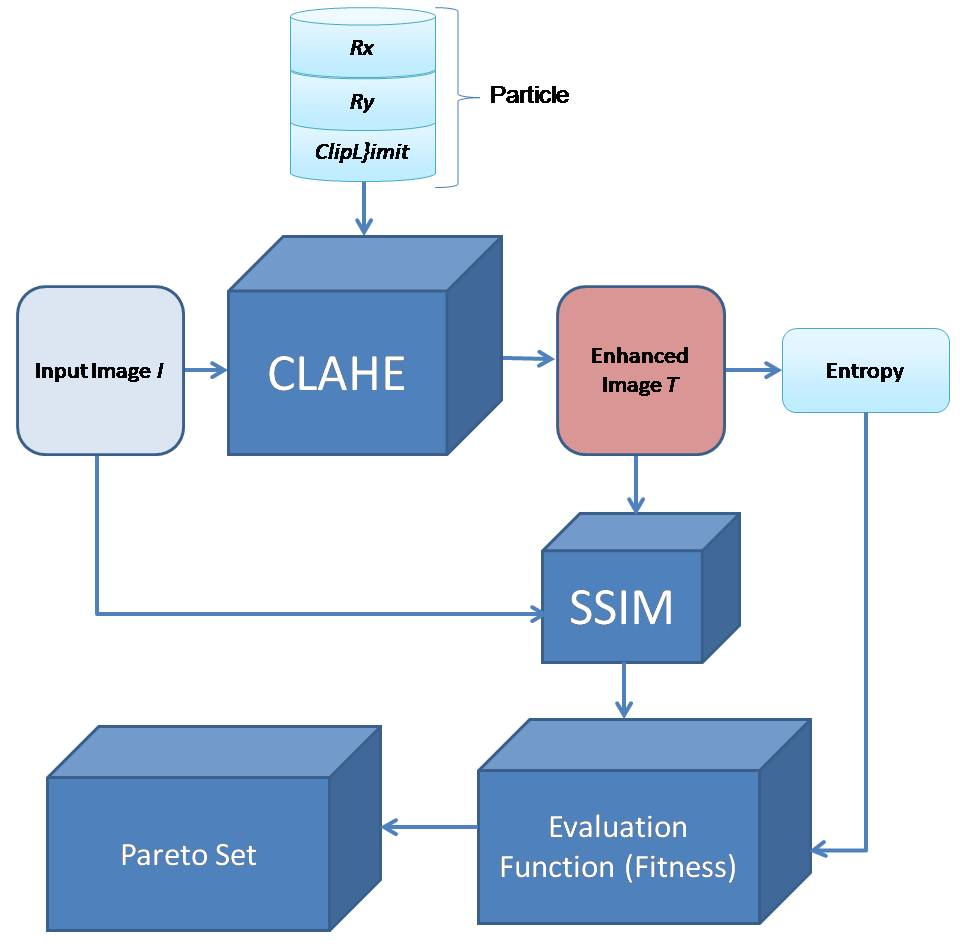
\includegraphics[height=7cm]{Figures/particula_clahe2}}
  \vspace{0.4cm}
  \label{fig:particula_clahe}
  \captionof{figure}{Interaction between $CLAHE$ and $MOPSO$ particle.}
\end{minipage}

\section{Results and Discussion}
\label{sec:resultadosdiscusion}

 Tests were performed using 16 images of chest radiographs and mammography, in order to assess the effectiveness of this proposal; they were downloaded from http://openi.nlm.nih.gov/. $SMPSO$ implementation is available at \cite{5586354}, meanwhile the corresponding implementations of $CLAHE$, $\mathscr{H}$ and $SSIM$ are available at \cite{opencv_library}. The initial parameters chosen for $SMPSO$ are listed in \textbf{Table \ref{table:parametrospso}}.


\begin{table}[h]
\begin{center}
 \begin{tabular}{||c c | c c||} 
 \hline
 Parameter & Value & Parameter & Value \\ [0.5ex] 
 \hline\hline
 $lower\_limit_{\mathscr{R}_x}$ & $2$ & $upper\_limit_{\mathscr{R}_x}$ & $M/2$ \\ 
 \hline
 $lower\_limit_{\mathscr{R}_y}$ & $2$ & $upper\_limit_{\mathscr{R}_y}$ & $N/2$ \\  
 \hline
 $lower\_limit_{{\mathscr{C}}}$ & $0$ & $upper\_limit_{{\mathscr{C}}}$ & $0,5$ \\
\hline
$\Omega$ & $100$ & $t_{max}$ & $100$ \\ 
\hline
$C_1$ $min$ & $1,5$ & $C_1$ $max$ & $2,5$ \\ 
\hline
$C_2$ $min$ & $1,5$ & $C_2$ $max$ & $2,5$ \\ 
\hline
$r_1$ $min$ & $0,0$ & $r_1$ $max$ & $1,0$ \\ 
\hline
$r_2$ $min$ & $0,0$ & $r_2$ $max$ & $1,0$ \\ [1ex]
\hline
\end{tabular}
\end{center}
\caption[Parámetros de entrada para $SMPSO$]{Initial parameters for $SMPSO$.}
\label{table:parametrospso}
\end{table}
 
 For every test image, 30 executions of $MOPSO-CLAHE$ were performed. Approximately 300 Pareto solutions were obtained for every image, which represents a wide group of images at different levels of contrast and distortion, thereby facilitating further analysis. In \textbf {Fig. 2,3,4} there are 2 of the Pareto set solutions, in order to visually assess how contrast varies, and also the original image as reference. In \textbf {Fig. 2c,3c,4c} it is noteworthy that there is an inverse relationship between objectives, this is, when $\mathscr{H}$ is increased, the $SSIM$ coefficient decreases; this means that both metrics are complementary in order to maintain the compromise between contrast enhancement and distortion minimization. From the Pareto set it is possible to obtain images which allow to visualize different details while the contrast changes. It is also remarkable that the soft tissues are better seen in chest radiographs when certain contrast is reached (see \textbf {Fig. 2b,4b}). A similar effect is achieved in mammograms (see \textbf {Fig. 3b}), in which potential injuries are more visible, but the fine details are preserved successfully. In this proposal, a significant amount of resulting images are obtained, with different relations between contrast and distortion, in an automatic manner, which represents an advantage because it can lead to better diagnoses.


\section{conclusions}
\label{sec:conclusion}
A multiobjective meta-heuristic algorithm is presented which maximizes simultaneously contrast by means of Entropy and Structural Similarity Index; with the latter it is possible to minimize image distortion, in medical images context, specifically in chest radiographs and mammograms. Experimental results show a set of solutions at different contrast levels, and allowing to highlight different structures. This would allow medical specialists to handle different visualization options automatically, which is useful for diagnostics.

The authors are still executing tests with several images found in the search engine. As future work it might be useful to adopt new meta-heuristics, such as multi-objective genetic algorithms, and take into account metrics based in high order statistics, as seen in \cite{7056527}, and local saliency maps based metrics, as in \cite{LTG}.




% References should be produced using the bibtex program from suitable
% BiBTeX files (here: refs). The IEEEbib.bst bibliography
% style file from IEEE produces unsorted bibliography list.
% -------------------------------------------------------------------------
\onecolumn
\noindent\begin{minipage}[b]{1.0\linewidth}
  \centering
   
   \begin{minipage}[t]{0.3\linewidth}  
   		\centering
        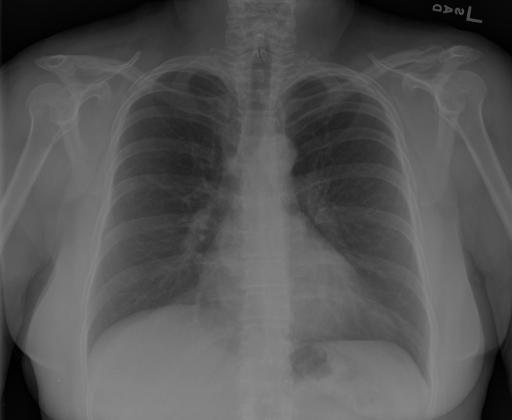
\includegraphics[width=4.1cm]{Figures/100_IM-0002-1001.png}
   		\captionof{subfigure}{Original Image}
  	\end{minipage}
  \hspace{1pt}
   \begin{minipage}[t]{0.3\linewidth}  
   		\centering
        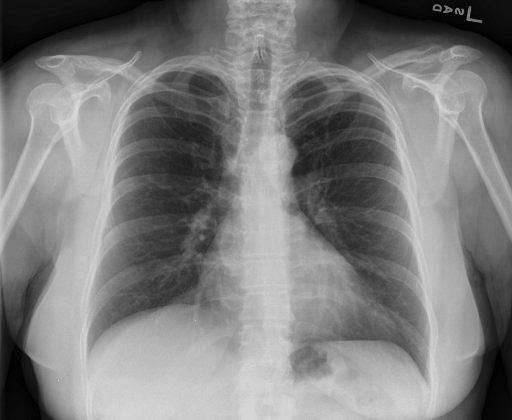
\includegraphics[width=4.1cm]{Figures/1182-100_IM-0002-1001.png}
   		\captionof{subfigure}{Resultant Image. $SSIM=0.9688$ $\mathscr{H}=0.7922$}
  	\end{minipage}
  \hspace{1pt}
   \begin{minipage}[t]{0.3\linewidth}  
   		\centering
        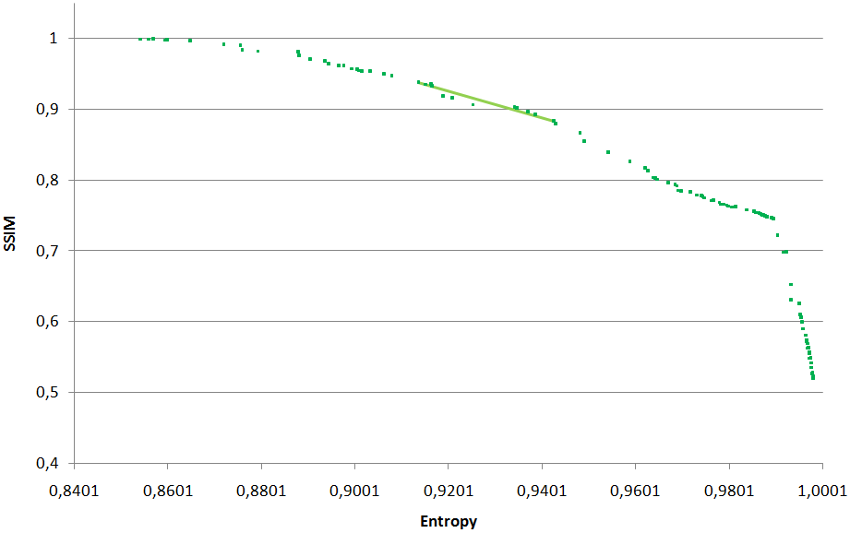
\includegraphics[width=6cm]{Figures/pareto_100_IM-0002-1001.png}
   		\captionof{subfigure}{Pareto front graphic related to this image.}
  	\end{minipage}
  \vspace{0.5cm}
    \label{fig:resultado1}
  \captionof{figure}{Result of multi-objective $PSO-CLAHE$. }

\end{minipage}

\begin{minipage}[b]{1.0\linewidth}
  
   \begin{minipage}[t]{0.3\linewidth}  
   		\centering
        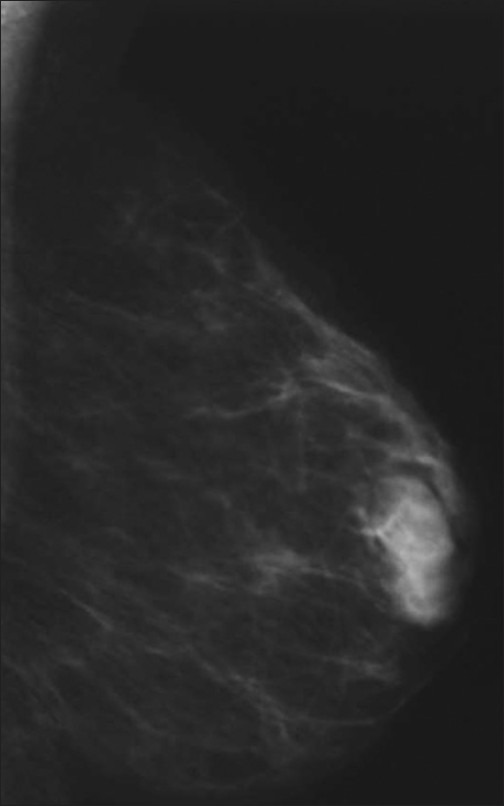
\includegraphics[width=3cm]{Figures/3715982_IJMPO-34-47-g001.png}
   		\captionof{subfigure}{Original Image}
  	\end{minipage}
  \hspace{1pt}
   \begin{minipage}[t]{0.3\linewidth}  
   		\centering
        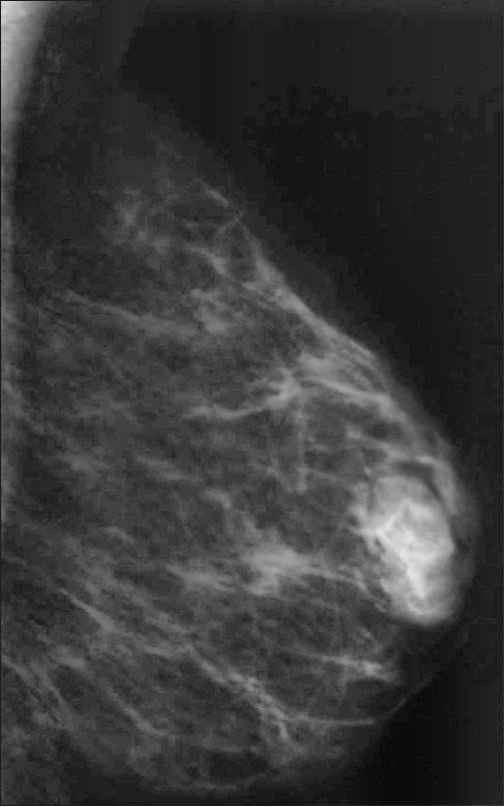
\includegraphics[width=3cm]{Figures/11608-3715982_IJMPO-34-47-g001.png}
   		\captionof{subfigure}{Resultant Image. $SSIM=0.8032$ $\mathscr{H}=0.8549$}
  	\end{minipage}
    \vspace{0.5cm}
   \begin{minipage}[t]{0.3\linewidth}  
   		\centering
        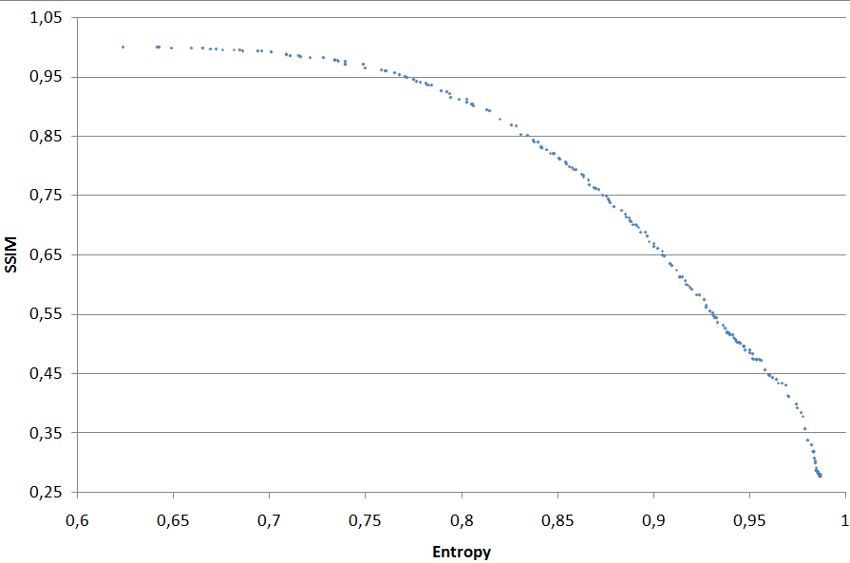
\includegraphics[width=7cm]{Figures/pareto_IJMPO-34-47-g001.png}
   		\captionof{subfigure}{Pareto front graphic related to this image.}
  	\end{minipage}
  \vspace{0.5cm}
    \label{fig:resultado2}
  \captionof{figure}{Results of multi-objective $PSO-CLAHE$. }

\end{minipage}

\begin{minipage}[b]{1.0\linewidth}
  
   \begin{minipage}[t]{0.3\linewidth}  
        \centering
        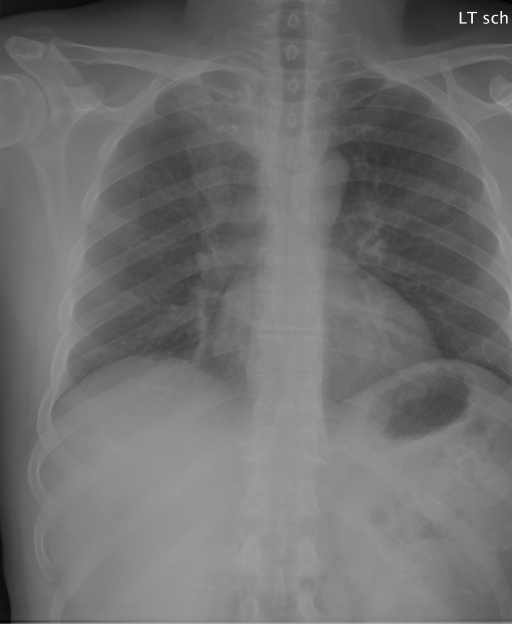
\includegraphics[width=3cm]{Figures/1000_IM-0003-1001.png}
        \captionof{subfigure}{Original Image}
    \end{minipage}
  \hspace{1pt}
   \begin{minipage}[t]{0.3\linewidth}  
        \centering
        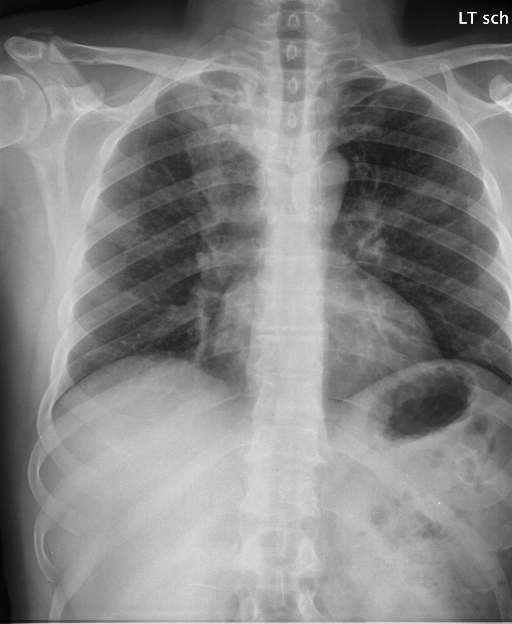
\includegraphics[width=3cm]{Figures/8178-1000_IM-0003-1001.png}
        \captionof{subfigure}{Resultant Image. $SSIM=0.8423$ $\mathscr{H}=0.9528$}
    \end{minipage}
    \vspace{0.5cm}
   \begin{minipage}[t]{0.3\linewidth}  
        \centering
        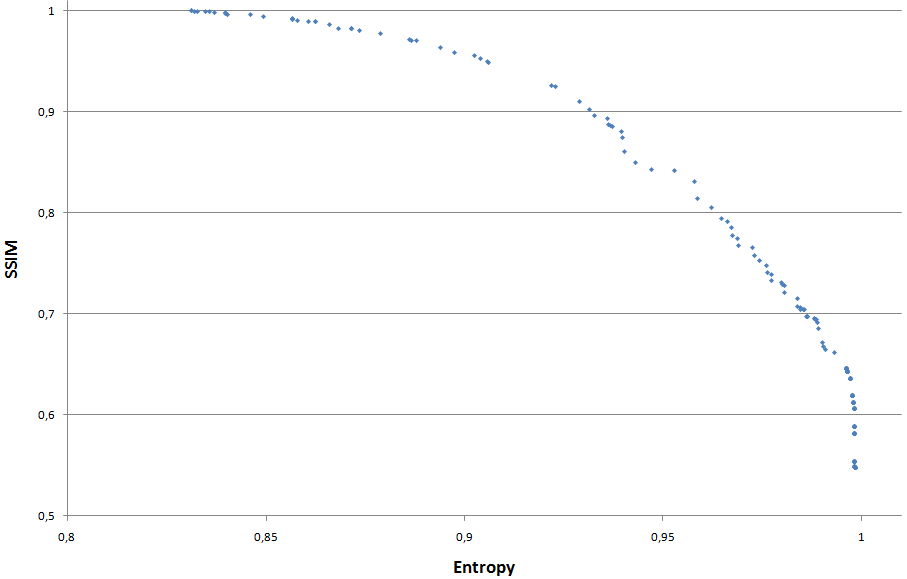
\includegraphics[width=7cm]{Figures/pareto_1000_IM-0003-1001.png}
        \captionof{subfigure}{Pareto front graphic related to this image.}
    \end{minipage}
  \vspace{0.5cm}
    \label{fig:resultado2}
  \captionof{figure}{Results of multi-objective $PSO-CLAHE$. }

\end{minipage}

% \begin{minipage}[b]{1.0\linewidth}

%    \begin{minipage}[b]{1.0\linewidth}  
%    		\centering
%         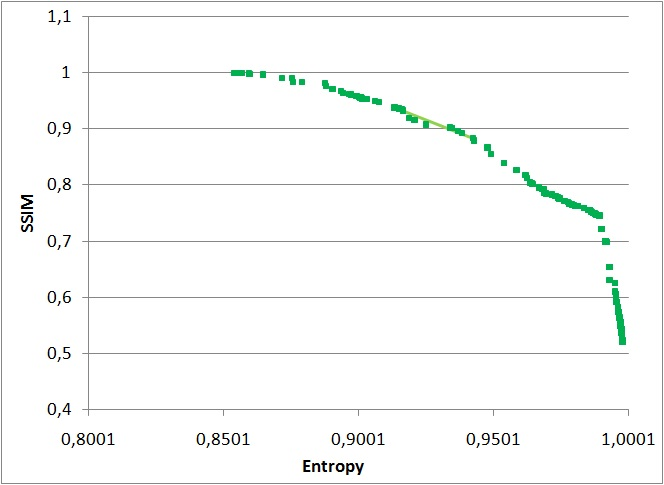
\includegraphics[height=7.5cm]{Figures/pareto-chest.jpg}
%    		%\captionof{subfigure}{Frente Pareto de la \textbf{Fig. 2}}
%   	\end{minipage}
%    \hspace{1pt}
%   % \begin{minipage}[b]{0.48\linewidth}  
%   % 		\centering
%   %      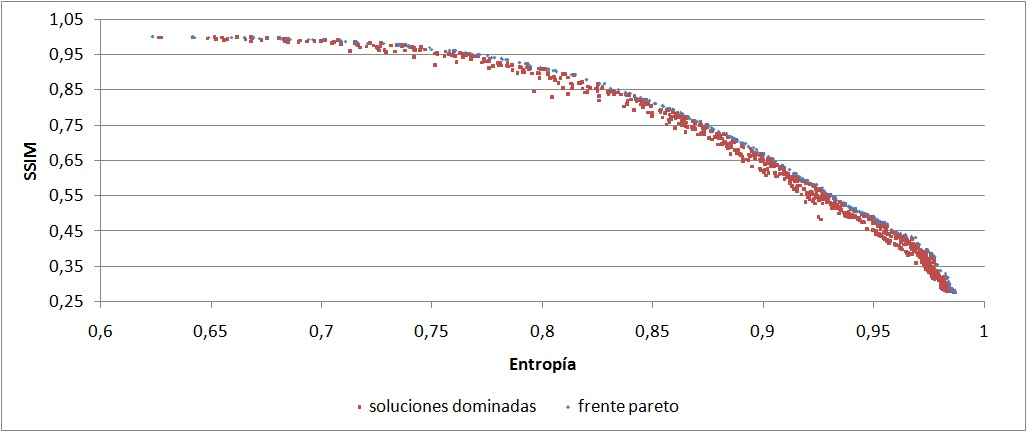
\includegraphics[height=6cm, width=10cm]{Figures/pareto-mamografia.jpg}
%   % 		\captionof{subfigure}{Frente Pareto de la \textbf{Fig. 3}}
%   %	\end{minipage}
%   \vspace{0.5cm}
%     \label{fig:resultado3}
%   \captionof{figure}{Pareto front for the images of  \textbf {Fig. 2}}.

% \end{minipage}


\twocolumn
%\bibliographystyle{IEEEbib}
\bibliographystyle{ieeetr}
\bibliography{refs}



\end{document}
